%!TEX root = ../kr.tex
%\chapter{Платформи оголошень та цифрові псевдопослуги}

\chapter{Види шахрайських схем на платформах оголошень}

\term{Онлайн-платформи} для купівлі-продажу товарів і послуг (наприклад, \example{OLX, Prom, Rozetka Market}, міжнародні \term{маркетплейси}) є дуже популярними серед користувачів. Цим активно користуються \important{шахраї}, які створюють \term{фейкові оголошення} або підроблені акаунти\footnote{Особистий кабінет користувача на сайті.} для виманювання коштів та персональних даних. 


\vspace{0.3cm}
%\noindent\textbf{Продаж неіснуючих товарів}
\section{Продаж неіснуючих товарів}

Найпоширеніша схема — фейкові оголошення про продаж популярних товарів, яких насправді не існує. Це можуть бути смартфони, ноутбуки, квитки на концерти, побутова техніка. «Обіцяна вигода» завжди виглядає переконливо: товар на 30–40\% дешевший, «розпродаж залишків», «потрібно терміново гроші». Жертва надсилає передоплату — і продавець зникає.

\example{Наприклад,} у лютому 2023 року співробітники кіберполіції Києва викрили \term{організовану групу}, учасники якої на онлайн-платформах оголошень ошукували громадян під виглядом продажу мобільної та комп'ютерної техніки. Зловмисники вимагали від покупців повну передоплату на банківські картки, а після отримання коштів припиняли зв'язок або блокували клієнтів (Департамент кіберполіції, 2023).

\vspace{0.3cm}

\section{Фейкова оренда житла}

Ще одна популярна схема — «оренда-примара». Оголошення про дешеву квартиру з привабливими фото, які часто скопійовані з реальних сайтів нерухомості. Так званий «Власник» просить невеликий завдаток, щоб забронювати житло, але після переказу коштів зникає. Найчастіше жертвами стають студенти або внутрішньо переміщені особи, які потребують житла, шукаючи його в дуже короткий проміжок часу.

\vspace{0.3cm}
\section{Фіктивні послуги}

Шахраї пропонують ремонт, доставку, навчання, допомогу з працевлаштуванням, курси за передоплатою тощо. Після отримання грошових коштів будь-який зв’язок припиняється. Під час дефіциту генераторів у 2022–2023 рр. такі оголошення масово з’являлися на платформах. Люди відправляли «символічні» 500–1000 грн, щоб забронювати товар, але втрачали їх.

\textit{Яскравий приклад,} на Київщині правоохоронці викрили організовану групу, яка створила мережу фейкових вебсайтів із продажу генераторів. 

Користуючись панічним попитом під час блекаутів\footnote{Від англ. blackout — «затемнення». Масове відключення електроенергії на великій території.}, зловмисники переконували покупців з усієї України робити повну передоплату. У результаті 33 потерпілих втратили понад 1,2 млн гривень (Київська обласна прокуратура, 2024).

\vspace{0.3cm}
\section{Як працює «OLX-доставка» у шахрайській версії:}

\begin{enumerate}
    \item Шахрай пише продавцю або покупцю, пропонуючи «оформити через сервіс доставки».
    \item Надсилає фішингове покликання\footnote{Підроблене покликання з метою обману.}, яке зовні імітує офіційний сайт.
    \item Жертва вводить реквізити\footnote{Дані про картку, необхідні для переказу грошей (номер, CVV, строк дії).} банківської картки.
    \item Дані потрапляють шахраям, і кошти миттєво списуються.
\end{enumerate}

\important{Порада:} \term{ніколи не переходьте за покликаннями}, отриманими в месенджерах. Усі дії здійснюйте лише з \keyword{офіційного сайту} OLX або мобільного застосунку.

\vspace{0.3cm}
\section{Маніпуляція довірою}

Шахраї не лише технічно хитрі, а й психологічно точні. Вони грають на:
\begin{enumerate}
    \item Терміновості («це останній екземпляр», «велика черга на товар»).
    \item Почутті вигоди (занадто низька ціна знімає скепсис).
    \item Ілюзії безпеки (згадка відомої служби доставки створює уявну легальність).
    \item Малих сум — «символічна» передоплата здається безпечною, але відкриває доступ до карткових даних користувача (див. табл.~\ref{tab:table1}).
\end{enumerate}

\newpage

Як це виглядає на практиці:

\begin{table}[H]
    \centering
    \caption{Алгоритм реалізації шахрайської схеми}
    \label{tab:table1}
    % Використовуємо p{...} для автоматичного перенесення тексту
    \begin{tabular}{|>{\raggedright\arraybackslash}p{0.28\linewidth}|>{\raggedright\arraybackslash}p{0.28\linewidth}|>{\raggedright\arraybackslash}p{0.28\linewidth}|}
        \hline
        \multicolumn{1}{|c|}{\textbf{Дія шахрая}} & \multicolumn{1}{c|}{\textbf{Як реагує користувач}} & \multicolumn{1}{c|}{\textbf{Результат}} \\ \hline
        
        Публікує оголошення з низькою ціною & 
        Зацікавлення, бажання «встигнути» & 
        Зниження критичності \\ \hline
        
        Пропонує «OLX-доставку» або «бронювання» & 
        Вводить дані картки, переказує завдаток & 
        Втрата коштів \\ \hline
        
        Пише в месенджері, створюючи атмосферу довіри & 
        Не перевіряє покликання або профіль & 
        Дані потрапляють шахраям \\ \hline
        
        Зникає після отримання грошей & 
        Жертва блокує, звертається в банк/поліцію & 
        Гроші повернути майже неможливо \\ \hline
    \end{tabular}
\end{table}

% \vspace{0.3cm}
\noindent\important{Підсумок}

\term{Більшість схем шахраїв} на платформах оголошень побудовані на двох принципах — \keyword{передоплаті та емоційній маніпуляції}. Там, де спрацьовує поспіх і бажання «зекономити», зникає критичне мислення. \important{Захист простий}: не платити наперед, не переходити за сторонніми покликаннями і перевіряти все, що здається «занадто вигідним».

Щоб убезпечити себе від шахраїв, експерти та банки радять ніколи не переходити за покликаннями, які надсилають у месенджерах чи SMS (див. 1.10 та 1.11).

\newpage

\chapter{Підроблені профілі та фейкові товари (послуги)}

Шахраї часто маскуються під справжніх продавців, створюючи копії реальних профілів або акаунтів (облікових сторінок на сайті), які виглядають переконливо: з фото, відгуками та нібито «проданими товарами». Це створює ілюзію авторитетності, навіть якщо профіль існує лише кілька днів. Часто злочинці копіюють оголошення з реальних сторінок — ті самі зображення, описи, навіть ціни — і жертва впізнає «знайомий» контент, вважаючи його безпечним.

\vspace{0.3cm}

\section{Ситуація «Колекціонер» з Одеси}

В Одесі неодноразово фіксували діяльність чоловіка, який продавав популярні комп'ютерні ігри та аксесуари для консолей через \example{OLX}. Його профіль виглядав \term{переконливо}: фото товарів, коротка історія продавця — «колекціонер, що розпродає власну колекцію», — і навіть кілька позитивних відгуків.

Схема була простою: він домовлявся про купівлю, \important{вимагав передоплату 200–400 грн} і одразу зникав. Заблокований профіль швидко відновлювався під іншим іменем і з тими ж фото. \keyword{Маніпуляція} працювала безвідмовно: довіра до «реального» профілю плюс ефект терміновості («ігри швидко розкуповують») знижували пильність.

\newpage

\example{Висновок.} Тут спрацювало поєднання довіри до «людини з історією» та страху втратити вигідну можливість. Для підлітків, які є основною аудиторією геймінг-ринку, особливо характерний механізм штучного прискореного зближення (rapid bonding). Шахраї майстерно імітують спільні інтереси (ігри, хобі), щоб створити ілюзію безпеки. Це критично, оскільки префронтальна кора мозку підлітка, що відповідає за оцінку ризиків та контроль імпульсів, ще перебуває у стані активного формування, що робить їх біологічно вразливішими до таких маніпуляцій.

\vspace{0.3cm}
\section{Ситуація «Брендова косметика» зі столиці}

У Києві шахрайка під вигаданим ім’ям створила сторінку продавчині «брендової косметики». Фото виглядали професійно, описи — як у справжніх інтернет-магазинів. Вона переконувала покупців, що товар «у великому попиті» і «залишилася остання партія», вимагаючи передоплату для «бронювання». Насправді всі фотографії були взяті з офіційних сайтів, а гроші — на особисту картку. Після переказу зв’язок одразу припинявся.

\textit{Висновок.} Cпрацювали дві ключові пастки — видимість легітимності (реалістичний стиль профілю) та психологічний тиск часу («останній шанс»).

\newpage

\noindent\textbf{Типові маніпуляції та психологічні пастки шахраїв:}

\begin{enumerate}
    \item \textbf{Абсолютно вигідна ціна (штучна економія та ефект «знахідки»).} Зловмисники навмисно встановлюють вартість товару чи послуги на 30–50\% нижче за середньоринкову. Це викликає в споживача яскраву емоційну реакцію — жагу до швидкої наживи та відчуття власної винятковості. У такому стані вмикається тунельне мислення: людина повністю зосереджується на потенційній вигоді й прагне здійснити транзакцію якомога швидше, щоб «не втратити шанс». 

    \item \textbf{Імітація віртуальної авторитетності та соціальний доказ.} Акаунти зловмисників ретельно маскуються під легітимні бізнес-сторінки або брендові магазини. Профілі виглядають «живими» завдяки якісним фотографіям, великій кількості підписників, накрученим вподобанням, коментарям та численним «позитивним відгукам» від нібито задоволених покупців. Шахраї вдало експлуатують психологічний феномен соціального доказу: людина підсвідомо вірить переконливому вигляду сторінки. 

    \item \textbf{Штучний дефіцит, терміновість та синдром втраченої вигоди (FOMO).} Класичний психологічний тиск, спрямований на відключення раціонального аналізу через страх втрати. Шахраї активно використовують агресивні маркетингові тригери: \textit{«на цей товар уже є три покупці», «залишився останній примірник за такою ціною», «акційна пропозиція діє лише найближчі 15 хвилин»}. Такий штучний ажіотаж створює стресову ситуацію, позбавляє жертву часу на роздуми, пораду з близькими або незалежну перевірку інформації, змушуючи негайно переказувати завдаток чи розголошувати реквізити картки.

    \item \textbf{Псевдогарантії, маніпуляція довірою та імітація безпеки.} Аби присипити пильність покупця, зловмисники самі проявляють «ініціативу» щодо безпеки: пропонують скористатися «захищеною угодою», надсилають підроблені квитанції, фіктивні трек-номери або посилання на фішингові копії відомих сервісів доставки та платіжних систем. Візуально ці сторінки до дрібниць копіюють оригінальні ресурси, створюючи хибне відчуття захищеності, хоча насправді повністю контролюються шахраями для викрадення грошей або облікових даних.

    \item \textbf{Емоційні гойдалки та переключення ролей.} Якщо покупець починає вагатися або ставити уточнювальні запитання, шахраї миттєво змінюють тактику спілкування. Вони вдаються до роздратування, удаваної образи (\textit{«Ви мені не довіряєте? Я офіційний продавець!»}) або навпаки — демонструють надмірну доброзичливість і поступливість. Така зміна емоційного фону змушує людину почуватися ніяково та погоджуватися на умови зловмисника, аби уникнути конфлікту.
\end{enumerate}

\vspace{0.8em}

\noindent Системне застосування цих психологічних прийомів спрямоване на те, щоб вивести людину з стану рівноваги, блокувати критичне мислення та змусити її ухвалити рішення під впливом емоцій. Щоб убезпечити себе від шахрайських дій та завчасно розпізнати маніпуляції, варто завжди звертати увагу на ключові індикатори ризику, детально описані в розділі 1.6.

\newpage

\chapter{Схеми у сфері працевлаштування: «псевдороботодавців» та «псевдоробітників»}


Ринок праці на платформах оголошень є специфічним вектором атак, де шахраї експлуатують базову потребу людини в стабільному доході. Психологічний тиск тут будується на ілюзії «успішного відбору» та страху втратити вигідну вакансію.

Шахрайство у сфері працевлаштування не завжди спрямоване на безробітних. Часто жертвами стають підприємці та рекрутери\footnote{Фахівець із підбору персоналу.}, які шукають спеціалістів на віддалену роботу.

\vspace{0.3cm}
\section{Сценарій «Платне стажування або навчання»}

Жертві повідомляють, що вона успішно пройшла відбір, але перед початком роботи потрібно сплатити за методичні матеріали, отримати платний доступ до \term{CRM-системи}\footnote{Програмне забезпечення для керування відносинами з клієнтами.} або пройти обов'язковий сертифікований курс. \important{Суть обману:} після оплати «роботодавець» припиняє зв'язок, а обіцяна вакансія виявляється неіснуючою.

\example{Приклад із життя: «Вакансія копірайтера у великому холдингу»}

Олена знайшла привабливу вакансію «Дистанційний помічник редактора» у великому медіа-холдингу\footnote{Холдинг — сукупність материнської та дочірніх компаній, де головна фірма контролює діяльність інших.} із заробітною платою 25~000 грн. Після короткої співбесіди в Telegram їй повідомили: «Ви нам ідеально підходите, ваші тексти чудові! Ми готові зарахувати вас у штат». 

Проте виникла одна «технічна» дрібниця: для роботи в корпоративній системі \term{Bitrix24} або \term{Jira} потрібно активувати іменний ліцензійний ключ, який коштує 450 грн. «Роботодавець» запевнив, що ці гроші — лише застава, яку повернуть разом із першою зарплатою, а оплата потрібна лише для того, щоб підтвердити серйозність намірів працювати, адже «багато кандидатів зникають після отримання доступу до бази».

\textit{Результат.} Олена переказала кошти на картку «бухгалтера», після чого її акаунт у месенджері заблокували, а оголошення про вакансію видалили. 

Насправді великі компанії завжди самі оплачують робочі інструменти для своїх працівників.

\example{Висновок.}  Шахраї використали \important{ефект підтвердження успіху} — людина, яка щойно отримала бажану роботу, перебуває у стані ейфорії та легше погоджується на «незначні» витрати.

\vspace{0.3cm}
\section{Сценарій «Застава за інструменти»}

Ця схема актуальна для віддаленої роботи, пов'язаної з фізичною працею (збирання ручок, пакування подарунків, сортування товарів). Шахраї вимагають «страховий внесок» за розхідні матеріали чи обладнання, які нібито надішлють поштою. Мотивація — «гарантія, що ви не вкрадете товар». Насправді після переказу застави зловмисник зникає.

\example{Приклад із життя: «Справа про елітні подарункові бокси»}

Студент Максим знайшов у соціальній мережі оголошення про підробіток: «Складання святкових наборів удома». Робота здавалася простою: кур'єр привозить складники (коробки, стрічки, декор, елітний шоколад), Максим їх пакує за зразком, а наступного дня кур'єр забирає готові бокси й виплачує гонорар.

Під час листування «менеджер» пояснив: «Оскільки ми надаємо вам дорогі інгредієнти та фірмове пакування, компанія має бути впевнена, що ви не зникнете з товаром. Потрібно внести гарантійний платіж у розмірі 600 грн. Це чиста формальність — суму буде повернуто вам разом із першою оплатою за виконану роботу». Для переконливості Максиму надіслали фото «накладної» з логотипом відомої служби доставки.

\textit{Результат.} Максим переказав гроші на вказаний номер картки. Після цього «менеджер» повідомив, що кур'єр запізнюється, а за годину листування було повністю видалене шахраєм, а телефонний номер став недоступним. Ніяких товарів для пакування хлопець так і не отримав.

\example{Висновок.} Шахраї використовують \important{логічне виправдання} (захист майна компанії), щоб зняти підозру. Пам’ятайте: \keyword{серйозні підприємства} закладають ризики втрати товару в операційні витрати або використовують договори з паспортними даними, але ніколи не вимагають «страхових внесків» готівкою на картку.

\vspace{0.3cm}
\section{Сценарій «Оформлення через дзеркальний сайт»}

Найбільш небезпечний технічний сценарій. Кандидату надсилають покликання на фішингову сторінку, що імітує «департамент кадрів» або відомий банк. Під приводом «відкриття зарплатного рахунку» або «верифікації особи» жертву змушують ввести повні дані картки, включаючи \keyword{CVV-код}. Це дає шахраям повний доступ до наявних коштів людини.

\newpage

\example{Приклад із життя: «Зарплатна картка від відомого банку»}

Ігор отримав пропозицію роботи на посаду логіста в компанію, що займається міжнародними перевезеннями. Після успішної онлайн-співбесіди «HR-менеджер» надіслав йому повідомлення: «Для зарахування у штат нам потрібно відкрити вам корпоративний рахунок у нашому банку-партнері. Ось офіційне покликання для реєстрації в кабінеті співробітника та прив'язки вашої поточної картки для верифікації». Покликання вело на сайт, який за дизайном, кольорами та логотипами був ідентичною копією відомого українського банку. У формі реєстрації було поле «Прив'язка картки для зарплати», де Ігор ввів номер своєї картки, термін дії та \keyword{CVV-код}. Для «підтвердження особи» система попросила ввести код із SMS, який надійшов на телефон. 

\textit{Результат.} Як тільки Ігор ввів код, з його рахунку зникло 12 000 грн. Виявилося, що сайт мав адресу \texttt{privat24-recruitment.com} замість офіційної \texttt{privat24.ua}, а введений код із SMS був не для «реєстрації», а для підтвердження переказу коштів на сторонній гаманець.

\example{Висновок.} Це класичний \term{фішинг}. Шахраї використовують авторитет відомих брендів (банків), щоб приспати пильність. Пам'ятайте: \important{жодна офіційна реєстрація} не потребує введення CVV-коду або паролів із SMS для «підтвердження особи» чи «відкриття рахунку».

\newpage 

\vspace{0.3cm}
\section{Сценарій «Тестове як безкоштовна експлуатація»}

Хоча ця схема не завжди передбачає крадіжку грошей напряму, вона є формою інтелектуального шахрайства. Кандидату дають реальне комерційне завдання (переклад великого тексту, дизайн макета, написання коду) під виглядом «тестового завдання». Після отримання результату комунікація припиняється, а роботу використовують безкоштовно.

\example{Приклад із життя: «Дизайн-проєкт для неіснуючого бренду»}

Марина, дизайнер-фрілансер, відгукнулася на вакансію від «нового амбітного стартапу». HR-менеджер надіслав їй технічне завдання: «Розробити повний брендинг для лінійки органічної косметики (логотип, етикетки для 5 видів кремів, дизайн сторінки в Instagram)». Обсяг роботи був значним, але Марину запевнили, що це «фінальний етап відбору серед трьох найкращих кандидатів».

Через три дні Марина надіслала готові макети у високій якості. Менеджер відповів: «Дякуємо, передаємо арт-директору на розгляд». Після цього переписка припинилася, а вакансія зникла. За місяць Марина випадково побачила свої макети на полицях крамниці під іншою назвою бренду. 

\textit{Результат.} Дівчина витратила 20 годин робочого часу, не отримавши жодної оплати, а компанія безкоштовно отримала готовий дизайн-продукт.

\newpage 

\example{Висновок.} Щоб уникнути інтелектуального крадійства, \important{завжди додавайте на тестові роботи водяні знаки}, надсилайте макети у низькій роздільній здатності або використовуйте платформи для фрілансу з функцією «безпечної угоди», де тестові завдання оплачуються.

%\textit{Сценарії від «псевдоробітників»: атаки на бізнес:}

\begin{center}
    \rule{0.8\textwidth}{0.1pt} \\ \vspace{0.2cm}
    \textit{Сценарії від «псевдоробітників»: атаки на бізнес}
    \rule{0.8\textwidth}{0.1pt}
\end{center}
\vspace{0.1cm}

\section{Сценарій «Аванс за вихід на роботу»}

Кандидат успішно проходить онлайн-інтерв'ю, демонструє вражаюче портфоліо (зазвичай вкрадене у реального спеціаліста) і погоджується на умови. Проте одразу після «найму» він заявляє про фінансові труднощі: просить аванс за перший тиждень, кошти на ремонт ноутбука або на оплату інтернету, щоб почати працювати.
\textit{Результат.} Після отримання коштів «робітник» зникає, так і не приступивши до обов'язків.

\vspace{0.3cm}
\section{Сценарій «Шкідливе резюме» (Targeted Attack)}

Зловмисник відгукується на вакансію і надсилає файл із резюме або тестовим завданням. Замість звичайного документа (\texttt{.pdf} або \texttt{.docx}) він надсилає архів (\texttt{.zip}, \texttt{.rar}) або покликання на хмарне сховище, де знаходиться файл із подвійним розширенням (наприклад, \texttt{Resume.pdf.exe}). 
\textit{Технічна суть:} при відкритті такого файлу на комп'ютер рекрутера встановлюється \term{стилер}\footnote{Шкідлива програма для викрадення логінів, паролів та банківських даних.}, що дає шахраям доступ до корпоративної пошти, клієнтських баз або банківських рахунків компанії.


\section{Приклад із життя: «Дороге тестове завдання»}

Власник невеликої онлайн-крамниці розмістив оголошення про пошук адміністратора та контент-менеджера. Один із кандидатів продемонстрував високий рівень зацікавленості й надіслав власне «портфоліо» та виконане тестове завдання у вигляді зашифрованого ZIP-архіву, додавши пароль у повідомленні. Свою вимогу щодо пароля він пояснив «захистом авторських розробок від копіювання іншими роботодавцями». 

Прагнучи якнайшвидше оцінити роботу потенційного працівника, власник завантажив архів і розпакував його. Всередині містився файл із подвійним розширенням (наприклад, \texttt{Portfolio.pdf.exe}), маскований під звичайний документ. Одразу після його відкриття в фоновому режимі запустився шкідливий скрипт (Stealer), який миттєво викрав збережені в браузері сесійні токени (куки) та авторизаційні дані. Уже за годину зловмисники отримали повний доступ до корпоративного акаунта, а з прив’язаного рекламного кабінету крамниці було списано 15~000 грн на просування сторонніх сумнівних ресурсів.

\example{Висновок.} Процес найму персоналу — це критична точка входу для загроз цифрової безпеки бізнесу. 

\newpage 

\chapter{Сценарії невідповідності: маніпуляції характеристиками та станом товару}

Цей тип шахрайства базується на \important{дезінформації} щодо фізичних або технічних властивостей об’єкта продажу. На відміну від схем із повним зникненням продавця, тут покупець дійсно отримує товар, проте його реальна вартість та стан суттєво відрізняються від заявлених. 

\vspace{0.3cm}
\section{Візуальні маніпуляції (Фото-фейк) та приховані дефекти}

Найпростіший метод обману — використання професійних рендерів\footnote{Цифрове зображення, створене за допомогою 3D-моделювання.} або «стокових» фотографій нових виробів замість реальних знімків. Шахраї майстерно приховують сколи, подряпини, плями або сліди падіння за допомогою специфічних ракурсів, штучного освiтлення та графічних фільтрів.

\example{Ситуація з практики: «Замаскований дефект та пастка огляду на пошті».} 

Андрій давно шукав конкретну модель смартфона й знайшов на біржі оголошень привабливий варіант за ціною, нижчою за ринкову. На фотографіях пристрій виглядав бездоганно: дзеркальний дисплей, яскраве забарвлення й відсутність будь-яких подряпин. 

\newpage 

Продавець пояснив терміновість продажу потребою в коштах і охоче погодився надіслати телефон післяплатою. У відділенні пошти Андрій поспішав, адже позаду утворилася черга. Він увімкнув смартфон: екран засвітився стандартним білим привітанням, сенсор відгукувався, а в меню все працювало швидко. Андрій підписав накладну, оплатив товар та забран посилку. 

Проте вже вдома, при детальному розгляді та зміні фону робочого столу на темний або суцільний кольоровий, виявилися приховані дефекти. У верхньому куті дисплея чітко проглядалася жовта пляма — наслідок перегріву та деградації матриці. Крім того, сама рамка корпусу мала ледь помітну деформацію після падіння, через яку екран поступово відклеювався від основи. На якісних фотографіях в оголошенні продавець майстерно приховав ці вади: використав строкаті шпалери, підбрав кут зйомки із яскравим відблиском світла та прикрив вигнутий край градієнтним чохлом.

Коли Андрій зателефонув продавцю, той категорично відмовився від повернення коштів, зайнявши жорстку позицію: \textit{«Ви особисто оглянули та перевірили телефон у відділенні пошти, підписали документ про відсутність претензій і добровільно внесли оплату. Після залишення відділення відповідальність за пристрій повністю лежить на вас»}. Юридично та формально оператор поштової служби також не мав підстав прийняти товар назад після завершення транзакції.

\vspace{0.3cm}

\important{Уроки цифрової гігієни та правила огляду техніки:}
\begin{itemize}
    \item \textbf{Не піддавайтеся часовому тиску:} Черга чи квапливість працівників пошти не повинні впливати на якість огляду. Перевірка дорогої техніки — це ваше право, за яке ви сплачуєте кошти.
    \item \textbf{Перевіряйте матрицю на різних фонах:} Завжди перевіряйте екран смартфона чи ноутбука на суцільно білому, чорному, червоному, зеленому та синьому фонах (для виявлення битих пікселів, «вигорання» AMOLED-матриць та жовтих плям від перегріву).
    \item \textbf{Оглядайте геометрію корпусу:} Знімайте всі чохли та захисні плівки, оглядайте торці пристрою під кутом уздовж граней для виявлення вигинів, щілин або слідів повторного склеювання.
    \item \textbf{Тестуйте функціонал повністю:} Перевіряйте роботу камер, мікрофонів, динаміків, бездротових модулів (Wi-Fi, Bluetooth, GPS), а також швидкість заряджання перед підписанням документів.
\end{itemize}

\section{Програмні маніпуляції та «Параметричний фейк» (Fake Capacity)}

Технічно складний вид шахрайства, поширений серед накопичувачів (флешки, SSD, жорсткі диски) та смартфонів. Зловмисники втручаються в \term{прошивку}\footnote{Прошивка — вбудоване програмне забезпечення пристрою.} контролера, щоб він повідомляв операційній системі неправдиві дані про об’єм пам’яті або модель процесора.

\example{Приклад.} Покупець придбав зовнішній SSD-накопичувач на 2~ТБ за дуже вигідною ціною. Комп’ютер дійсно відображав 2~терабайти вільного місця. Проте після запису перших 32~ГБ даних нові файли почали затирати попередні або ставали нечитабельними. Після розбирання корпусу з’ясувалося, що всередині була звичайна дешева флеш-карта на 32~ГБ, а контролер був програмно «обманутий» для імітації великого об’єму.

\newpage 
\section{Маніпуляції з комплектацією та «аксесуарна підміна»}

Оголошення зазвичай обіцяє «повний заводський комплект» (оригінальна коробка, документи, фірмові навушники та зарядний пристрій). На практиці шахрай вилучає оригінальні дорогі аксесуари, замінюючи їх на дешеві та низькоякісні копії («репліки»), або взагалі не додає їх до посилки. Це не лише знижує вартість покупки, а й може призвести до виходу техніки з ладу через невідповідні параметри живлення.

\example{Ситуація з практики: «Небезпечний зарядний пристрій та підміна комплектних аксесуарів».}

Олександр придбав на популярному маркетплейсі флагманський смартфон відомого бренду за дуже привабливою ціною. У тексті оголошення та на світлинах продавець наголошував: \textit{«Телефон у стані нового, повний заводський комплект із оригінальною швидкою зарядкою, фірмовим кабелем та гарнітурою»}. 

Оскільки посилка вирушала післяплатою з можливістю огляду, Олександр прийшов до відділення поштової служби. Він перевірив зовнішній вигляд смартфона, увімкнув його, переконався у відсутності блокування операторів і швидко підписав документи, розрахувавшись за замовлення. У шаленому темпі робочого дня він навіть не заглянув углиб коробки, де під картонним ложементом лежали аксесуари.

Справжні проблеми виникли вже вдома. Під час спроби підключити телефон до комплектного блоку живлення через фірмовий кабель смартфон видав попередження про системну помилку живлення, а за кілька хвилин корпус адаптера нагрівся до критичної температури та почав видавати специфічний запах плавленої пластмаси. Олександр одразу вимкнув пристрій із розетки. 

\newpage 

Детальний огляд аксесуарів виявив класичну підміну:
\begin{itemize}
    \item \textbf{Блок живлення} виявився кустарною дешевою підробкою візуально схожого дизайну, проте всередині нього була відсутня будь-яка плата стабілізації напруги чи захисту від перенапруги. Замість заявлених брендом 67 Вт такий пристрій видавав нестабільні стрибки струму, здатні миттєво спалити контролер живлення в материнській платі смартфона.
    \item \textbf{USB-кабель} мав занадто тонкі внутрішні мідні жили, які фізично не могли передати високий струм для швидкої зарядки, через що процес заряджання тривав понад шість годин.
    \item \textbf{Фірмові навушники}, заявлені як оригінальні, виявилися найдешевшою китайською копією з жахливим звучанням та крихким пластиком, який зламався при першому ж згинанні дна.
\end{itemize}

Коли Олександр звернувся до продавця з вимогою повернути частину коштів за неякісний і небезпечний комплект, той відповів стандартною фразою: \textit{«Ви оглядали посилку на пошті, телефон забрали, комплект вас влаштовував, я продавав усе як є»}. Продавець навмисно розраховував на те, що покупці детально перевіряють лише сам гаджет, повністю ігноруючи перевірку маркування, ваги та сертифікації комплектних аксесуарів.

\vspace{0.8em}

\important{Уроки цифрової гігієни та правила перевірки комплектації:}
\begin{enumerate}
    \item \textbf{Зважуйте та оглядайте кожну деталіку:} Оригінальні блоки живлення флагманських смартфонів завжди мають відчутну вагу завдяки наявності трансформаторів і захисних схем. Надто легкі, пластмасові адаптери з розмитими шрифтами на корпусі — пряма ознака підробки.
    \item \textbf{Звіряйте серійні номери:} На коробці, самому смартфоні та наклейках зарядних пристроїв штрихкоди й серійні номери зазвичай збігаються (або перевіряються через офіційні сервіси підтримки).
    \item \textbf{Не ризикуйте технікою заради економії на аксесуарах:} Використання контрафактних зарядних блоків — одна з найпоширеніших причин вибуху акумуляторів, виходу з ладу контролерів живлення та повної поломки дорогих смартфонів. Краще придбати якісний сертифікований аналог відомого стороннього бренду, ніж ризикувати оригінальним гаджетом.
\end{enumerate}

\section{Зворотна маніпуляція: споживче шахрайство та «Refund Fraud»}

Варто зауважити, що жертвою маніпуляцій може стати і продавець. «Споживче шахрайство» має на меті приховати власну необачність або отримати товар безкоштовно (чи з великою знижкою) через психологічний тиск та маніпуляцію правом на повернення.

\example{Ситуація з практики.} Власниця онлайн-магазину відправила клієнтці дорогу куртку з екошкіри післяплатою. Клієнтка оглянула товар у відділенні пошти, оплатила повну вартість і забрала пакунок. Проте вже за годину вона зателефонувала продавцеві в стані сильної емоційної напруги. Клієнтка стверджувала, що вдома виявила довгий вертикальний розріз на спині куртки, і миттєво перейшла до погроз: \textit{«Ви підсунули мені брак! Я напишу про вас у всіх групах, звернуся до поліції та захисту прав споживачів! Поверніть гроші негайно!»}. На надісланих фото дійсно було видно рівний розріз, проте він мав характерний вигляд сліду від канцелярського ножа.

\newpage 

\textbf{Аналіз події.} Найімовірніше, покупець випадково пошкодив річ під час необережного розпакування ножем удома. Усвідомивши помилку, він намагається перекласти відповідальність на продавця. Агресія в такому разі виступає інструментом «захисту через напад», щоб змусити продавця виправдовуватися і прийняти пошкоджену річ назад.

\vspace{0.1cm}
\textbf{Повчальний висновок для продавця:}
\begin{enumerate}
    \item \textbf{Презумпція цілісності.} Оплата товару та вихід із відділення пошти означає, що покупець підтвердив відсутність претензій. 
    \item \textbf{Архів пакування.} Відеофіксація процесу складання замовлення, де видно цілісність товару, є найкращим доказом у подібних суперечках.
    \item \textbf{Протокол реагування.} Не піддавайтеся на шантаж. Спокійно нагадайте клієнту, що огляд має проводитися в присутності працівника пошти із заповненням відповідного акта.
\end{enumerate}

\noindent\keyword{Як не стати жертвою маніпуляцій (поради для обох сторін):}

\begin{itemize}
    \item \textbf{Перевірка фото.} Вимагайте «живі» фото товару на фоні аркуша з поточного датою або специфічним написом.
    \item \textbf{Технічний контроль.} При покупці накопичувачів використовуйте утиліти типу \texttt{H2testw} для перевірки реальної ємності.
    \item \textbf{Принцип огляду на місці.} Будь-які претензії щодо зовнішнього вигляду та цілісності мають фіксуватися виключно у відділенні пошти. 
    \item \textbf{Звертайте увагу на деталі.} Сліди на гвинтах, стан гарантійних пломб та відповідність \term{IMEI}\footnote{International Mobile Equipment Identity — міжнародний ідентифікатор мобільного обладнання.} на екрані та на корпусі.
\end{itemize}

\newpage 

\chapter{Використання передоплати та фальшивих договорів}

Передоплата — найпоширеніша пастка онлайн-торгівлі. Саме через неї щодня тисячі користувачів втрачають гроші на платформах оголошень. Шахраї чудово знають: бажання «забронювати товар» або «встигнути придбати вигідну річ» сильніше за обережність.  

Щоб надати своїм діям вигляду легальності, шахраї часто надсилають фальшиві документи — «договір купівлі-продажу», «квитанцію» або навіть «фото паспорта продавця». Такі «папери» створюють у жертви відчуття офіційності, хоча в реальності це — випадкові зразки з інтернету або підроблені з використанням шаблонів. Ключовий прийом тут — створити ілюзію формальності, щоб покупець перестав сумніватися.

\section{Типовий сценарій}

Найчастіше все починається з невинного діалогу в чаті платформи оголошень. Потенційний покупець або продавець під різними приводами (наприклад, «тут погано завантажуються фотографії», «мені зручніше спілкуватися в месенджері» чи «так швидше узгодити деталі відправки») намагається перевести спілкування у сторонній месенджер\footnote{Програма в телефоні для листування та дзвінків.} — Telegram, Viber або WhatsApp. 

\newpage 

Щойно контакт встановлено, зловмисник надсилає посилання, яке ретельно замасковане під офіційну сторінку «OLX Доставка», «Нова пошта Pay» або відомий банківський сервіс. Дизайн ресурсу відтворено з досконалою точністю: знайомі корпоративні логотипи, фірмові кольори, шрифти, елементи інтерфейсу та навіть імітація живого чату технічної підтримки, яка нібито супроводжує транзакцію.

Жертва, бачачи звичний інтерфейс\footnote{Зовнішній вигляд сайту чи програми} та не помічаючи підступу в адресному рядку браузера (де доменне ім’я може відрізнятися лише однією літерою чи містити сторонні символи), втрачає пильність. Переконана в безпеці своїх дій, вона вводить повні реквізити власної банківської картки — номер, термін дії, тризначний CVV-код, а іноді й пін-код чи одноразові SMS-паролі від банку — і натискає кнопку підтвердження. Кошти списуються з рахунку миттєво. Щойно людина усвідомлює, що стала жертвою фішингу, зловмисник зазвичай зникає: акаунт у месенджері блокується чи видаляється, номери телефонів стають недоступними, а викрадені гроші за лічені хвилини розсипаються через сервіси транзиту або криптовалютні біржі на десятки різних рахунків. Така схема є надзвичайно небезпечною не лише з технічного боку, а й через психологічний вплив: бездоганна візуальна копія сервісу та «службовий» тон листування повністю притупляють природну настороженість людини, змушуючи її добровільно віддати доступ до власних фінансів.

\newpage 

\section{Приклад із реального життя}

Мешканець Сумського регіону виставив на продаж побутову техніку через OLX. Пропозиція була цілком звичайною, тому коли покупець запропонував «оформити через OLX Доставку», чоловік не підозрював нічого поганого. покликання, яке надійшло в месенджері, виглядало переконливо: логотипи, кольорова гама, навіть кнопка «Підтвердити оплату».

Продавець ввів дані картки — і вже за кілька хвилин з рахунку зникли всі гроші. Сайт виявився фішинговим клоном, створеним із мінімальними відмінностями в адресі (замість \texttt{olx.ua} — \texttt{olx-pay.com} або подібна варіація).

Ключовим моментом стало не технічне, а емоційне рішення. Людина, яка очікує оплату, перебуває у стані піднесення — серцебиття пришвидшується, мозок очікує винагороду. У цей момент критичність знижується: хочеться підтвердити операцію і «отримати гроші». Саме цю вразливу секунду використовують шахраї.

\vspace{0.3cm}
\noindent\textbf{Психологічні тригери:}

\begin{enumerate}
    \item \textbf{Терміновість.} «Покупець уже платить» або «залишилося лише натиснути» — створює відчуття, що діяти треба негайно.
    \item \textbf{Ілюзія безпеки.} Наявність «договору», «квитанції», «печатки» формує хибне відчуття контролю.
    \item \textbf{Ефект дрібної дії.} «Просто введіть номер картки» — здається безпечним кроком, але саме він запускає механізм крадіжки.
\end{enumerate}

У підсумку людина відчуває себе впевненою до останнього моменту, аж поки не отримує SMS із банку про списання коштів.

\vspace{0.3cm}\noindent\textbf{Історія з реального життя: Справа про iPhone і фальшивого кур'єра}

Юрій продавав свій iPhone 14 Pro Max на маркетплейсі Prom.ua. Техніка дорога, тому до покупців він ставився прискіпливо. Того дня йому написав клієнт — назвемо його Олег. Спілкування було ввічливим і стандартним: запитав про стан батареї та подряпини, а потім запропонував: «Давайте післяплатою через Нову Пошту?». Юрій погодився — це найбезпечніший спосіб для обох сторін.

\textit{Етап 1. Створення штучної проблеми.} 
Наступного дня телефон Юрія задзвонив. Це був той самий «покупець». Голос стурбований: «Добрий день! Слухайте, тут така проблема — у нас у відділенні на районі якийсь збій, термінали\footnote{Пристрій для оплати картками.} не працюють, черги шалені. Я не зможу забрати з відділення. Давайте оформимо адресну кур'єрську доставку? Я все оплачу». Юрій, хоч і здивувався, погодився, але для перестраховки сказав: «Добре, але я зараз зателефоную на гарячу лінію пошти, перевірю, як краще це оформити». Покупець швидко погодився і поклав слухавку.

\textit{Етап 2. Атака «кур'єра».} 
Минуло рівно півтори хвилини — Юрій навіть не встиг набрати номер підтримки. Вхідний дзвінок з невідомого номера. У слухавці пролунав молодий голос із дивним, наче награним, акцентом і дуже швидкою манерою мови: «Алло, добрий день! Це кур'єрська служба доставки. У вас там замовлення на iPhone змінюється на адресну. Зараз вам прийде SMS-код на телефон. Продиктуйте мені його, щоб я міг прийняти заявку і виїхати». Юрій напружився: «Чекайте, а навіщо код? Я просто відправляю товар». 

\newpage 

«Кур'єр» заторохтів: «Розумієте, покупець розраховується зі мною готівкою на місці. Я ці гроші проводжу через свій термінал, вони йдуть на відділення, а відділення вже зараховує їх вам на карту. Без коду система не пускає!».

\textit{Етап 3. Перевірка реальності.} Пояснення звучало як повна маячня. Схема «гроші–кур'єр–відділення–карта» була занадто складною для звичайної доставки. Юрій сказав: «Хвилинку, поганий зв'язок», — і поставив дзвінок на утримання. Він швидко скопіював номер «кур'єра» і вставив його в додаток GetContact та в пошук Google. Результат змусив його гірко посміхнутися. Теги в GetContact говорили самі за себе: «Шахрай ОЛХ», «Розвод на гроші», «Зек тюрма». В цей же момент на екрані спливло повідомлення від сервісу доставки: \textit{«Ваш код відновлення доступу до кабінету: 4921. НІКОМУ НЕ ПОВІДОМЛЯЙТЕ ЦЕЙ КОД, НАВІТЬ ПРАЦІВНИКАМ ПОШТИ»}. Усе стало на свої місця. Жодного кур'єра не існувало. Шахраї намагалися зламати особистий кабінет Юрія на сайті пошти або маркетплейсу, щоб підмінити реквізити для отримання грошей на свої власні.

\textit{Етап 4. Фінал.} Юрій зняв дзвінок з утримання. «Алло? Це Ростислав, кур'єр, ви ще тут? Код прийшов? Диктуйте, бо в мене графік!» — голос у трубці став наполегливішим. «Так, Ростислав, код прийшов, — спокійно відповів Юрій. — Там написано великими літерами: «Не повідомляти шахраям». Тож вибачте, «кур'єр», але сьогодні ви без зарплати». На тому кінці запала тиша, а потім «Ростислав» перейшов на добірну лайку, забувши про свій акцент, і кинув слухавку.

\textit{Висновок цієї історії.} Ця історія демонструє критичне мислення в дії. Шахраї створили штучний цейтнот (проблема з поштою → миттєвий дзвінок кур'єра), щоб не дати Юрію часу на роздуми. 

\newpage 

Але проста перевірка номера через GetContact та уважне читання тексту SMS (де завжди вказано призначення коду) врятували телефон вартістю в тисячу доларів. 

\textbf{Пам'ятайте!} Справжні кур'єри та працівники пошти ніколи не просять коди з SMS для оформлення доставки. Код — це ключ до ваших даних, а не до дверей кур'єра.

\vspace{0.3cm}\noindent\textbf{Підсумок}

Схеми з передоплатою та фальшивими договорами побудовані на ілюзії довіри та легітимності. Шахрай не зламує системи — він змушує людину самостійно віддати гроші, переконавши, що все «по правилах». Фальшивий договір, «квитанція» чи покликання від «служби доставки» — це не гарантія, а ознака небезпеки. Щоб убезпечити себе, варто пам’ятати головне правило:

\begin{quote}
\textit{{Майже жодна вигідна пропозиція не варта ризику передоплати. Оплату слід здійснювати тільки через офіційні сервіси платформи, без переходів за сторонніми покликаннями, навіть якщо вони виглядають «справжніми».}}
\end{quote}

\chapter{Механізми збору персональних даних}

Іноді шахраям не потрібні ваші гроші одразу — достатньо копії вашого паспорта. Платформи оголошень (наприклад, OLX) або торгові майданчики у соціальних мережах активно використовуються не лише для фішингу, але й для цілеспрямованого збору чутливих персональних даних. Схема часто виглядає невинно. Зловмисник, що видає себе за продавця або покупця, входить у довіру під час спілкування у приватному чаті.  У процесі обговорення угоди він просить надіслати фото документів (паспорта, ІПН\footnote{Реєстраційний номер облікової картки платника податків.}) чи повні реквізити картки нібито «для підтвердження особи», «перевірки надійності» або «оформлення доставки».

\section{Реальний приклад}

Саме так жертвою стала 42-річна мешканка Полтавської області. Під час купівлі дитячих речей у соцмережі вона надіслала «продавцю» фото паспорта для «підтвердження». Цей файл шахраї негайно використали для оформлення кількох мікропозик онлайн. Жінка дізналася про це лише за кілька місяців, коли їй почали телефонувати колектори\footnote{Люди, що вимагають повернути борг.} з вимогою повернути понад 60 тисяч гривень. Їй довелося місяцями доводити свою непричетність у судах, витративши значні кошти на юридичний захист і повністю зіпсувавши свою кредитну історію.

\newpage

\section{Навіщо збирають ці відомості?}

Отримані таким чином дані — скани документів, ІПН, адреси, номери карток — стають «сировиною» для десятків злочинних схем. Їх використовують для кредитного шахрайства, реєстрації фейкових акаунтів для нових атак або навіть для шантажу та вимагання.

Паспорт та ІПН (або РНОКПП) дозволяють дистанційно пройти верифікації\footnote{Процедура для підтвердження особи власника документів.}, відкривати акаунти і брати кредити. Адреса, телефон і e-mail (електронна пошта) дають поживу для наступних атак: підміна SIM і перехоплення SMS-кодів, візити «кур'єра» під двері, нові «підтвердження доставки». 

Повний номер картки разом із строком дії та CVV\footnote{Тризначний код безпеки на звороті банківської картки.} відкривають доступ до списань; одноразові коди з SMS або оповіщень додатка (push-повідомлень) завершують схему. Часто цю інформацію комбінують з іншими витоками — чим більше фрагментів, тим легше зібрати з них «цифровий портрет» і діяти від вашого імені.

\vspace{0.3cm}
\section{Типовий порядок подій}

Майже завжди однаковий: ви знаходите привабливе оголошення або самі публікуєте товар; співрозмовник пропонує перейти «туди, де зручніше» — у месенджер; надсилає «службову» форму для доставки чи повернення; просить «стандартні дані для підтвердження» і додає трохи терміновості — «черга на товар, давайте швидше». Знайомі логотипи та ввічлива манера спілкування знімають настороженість, і людина віддає більше, ніж потрібно.

\vspace{0.3cm}
\section{Як зрозуміти, що у вас виманюють дані?}

Вас підганяють («ще троє чекають»), просять надмірне для простої угоди («для доставки потрібні скани паспорта», «для повернення грошей дайте CVV»), переводять на зовнішній сайт із «правильним» виглядом, але іншим доменом\footnote{Адреса сайту в інтернеті.}, апелюють до безпеки та зручності («так усім спокійніше»). Ці маркери не про сервіс — вони про маніпуляцію. 

Зверніть увагу на наступні ознаки потенційної загрози:

\begin{enumerate}
     \item Якщо просять надати зайву інформацію для простої угоди: скан паспорта, ID\footnote{Документ, що посвідчує особу.} ІПН, селфі з документом, повний номер картки, строк дії, CVV або одноразові коди.
     \item Якщо пропонують перейти за покликанням із чату на сторінку, схожу на службу доставки чи банк; адреса сайту відрізняється від офіційної.
    \item Якщо поспішають і тиснуть у часі: «підтвердьте негайно», «ще кілька людей чекають», «акція завершується».
    \item Якщо посилаються на «стандартні правила» чи «службу безпеки», але відмовляються спілкуватися в офіційних чатах платформи або просити мінімум необхідних даних.
    \item Якщо вимагають IBAN\footnote{Міжнародний номер банківського рахунку для переказів.} або адресу доставки ще до підтвердження реальності угоди чи без очевидної потреби.
    \item Якщо у співрозмовника новий або «порожній» профіль, нечіткі відповіді, він уникає дзвінків і наполягає «вирішити все швидко в чаті».
\end{enumerate}

\newpage

\noindent Більш детально описано в підрозділі~1.6.



\vspace{0.3cm}
\noindent\textbf{Що тут критично запам’ятати:}

% Додаємо [label=\arabic*.] для примусового формату <<1. >>, <<2. >>
\begin{enumerate}[label=\arabic*.]
    \item \textbf{НЕ} надсилайте копії документів незнайомим.
    \item \textbf{НЕ} повідомляйте реквізити картки (номер, строк, CVV) та коди з SMS по телефону.
    \item \textbf{НЕ} надсилайте портретне фото з документа, адресу та IBAN для малознайомих чи підозрілих сервісів.
    \item \textbf{НЕ} переходьте за покликаннями з невідомих месенджерів.
    \item \textbf{НЕ} відкривайте невідомий сервіс, підозріле покликання через браузер\footnote{Спеціальна програма для входу в Інтернет.} або застосунок.
\end{enumerate}

\noindent Більш детально описано в підрозділі~1.11.

\vspace{0.3cm}
\section{Якщо вже надіслали дані}

Негайно: заблокуйте картку, змініть паролі до пошти, банкінгу та соцмереж, увімкніть двофакторну автентифікацію\footnote{Подвійний захист: пароль + код.}, забороніть у мобільного оператора перевипуск SIM\footnote{Картка з номером у телефоні.} без вашої присутності, перевірте кредитну історію, збережіть скріншоти\footnote{Фото екрана пристрою.} переписки й посилань та зверніться до банку і поліції. Швидкість тут критична: чим раніше ви обмежите використання даних, тим менше шансів на їхнє вторинне застосування.

\vspace{0.3cm}

\newpage

\noindent\textbf{Головне: загрози вторинного використання даних}

Втрата контролю над копіями паспорта, ідентифікаційного коду, сесійними токенами чи фотографіями з документами в руках неминуче призводить до серйозних юридичних та фінансових наслідків. На відміну від заблокованої банківської картки, яку можна перевипустити за кілька хвилин, наслідки компрометації ідентифікаційних даних доводиться розгрібати роками. Серед найбільш поширених сценаріїв вторинних атак:
\begin{itemize}
    \item \textbf{Оформлення мікрокредитів (Q-credits).} Шахраї використовують ваші документи для дистанційного відкриття швидких позик у небанківських фінансових установах (МФО), де перевірка позичальників є мінімальною. Про існування таких боргів людина зазвичай дізнається лише тоді, коли сума через величезні відсотки й штрафи зростає в десятки разів і справю починають колектори або виконавчі служби.
    \item \textbf{Реєстрація «дрібних» фіктивних компаній і криптовалютних гаманців.} Викрадені дані залучаються для створення акаунтів на біржах або реєстрації «транзитних» фірм-одноденевок (так званих «дропів»), через які відмиваються кошти, здобуті злочинним шляхом. У результаті власник паспорта стає формальним фігурантом кримінальних проваджень.
    \item \textbf{Серійний фішинг та соціальна інженерія.} Маючи на руках ваші справжні документи та історію попередніх взаємодій, зловмисники можуть видавати вас перед вашими родичами, колегами чи банками, здійснюючи нові, більш цілеспрямовані атаки.
\end{itemize}

Саме тому цифровизація документів вимагає підвищеної пильності.

\newpage

\chapter{Приклади відомих афер та статистика}

Шахрайство на платформах оголошень стало одним із найпомітніших явищ останніх років (рис.~\ref{fig:1_1}). Якщо у 2021~році збитки від незаконних дій із картками сягали близько 481~млн~грн, то вже у 2024~році масштаби суттєво зросли. За даними Національного банку України, у 2024~році сума збитків від шахрайських операцій перевищила 1,1~млрд~грн, що на 37\% більше, ніж роком раніше. При цьому 83\% усіх випадків шахрайства та 93\% загальної суми втрат припали саме на мережу Інтернет~\cite{NBU2025}.

\begin{figure}[H]
    \centering
    % Переконайтеся, що файл fig1_1.jpg (або png) є у папці img
    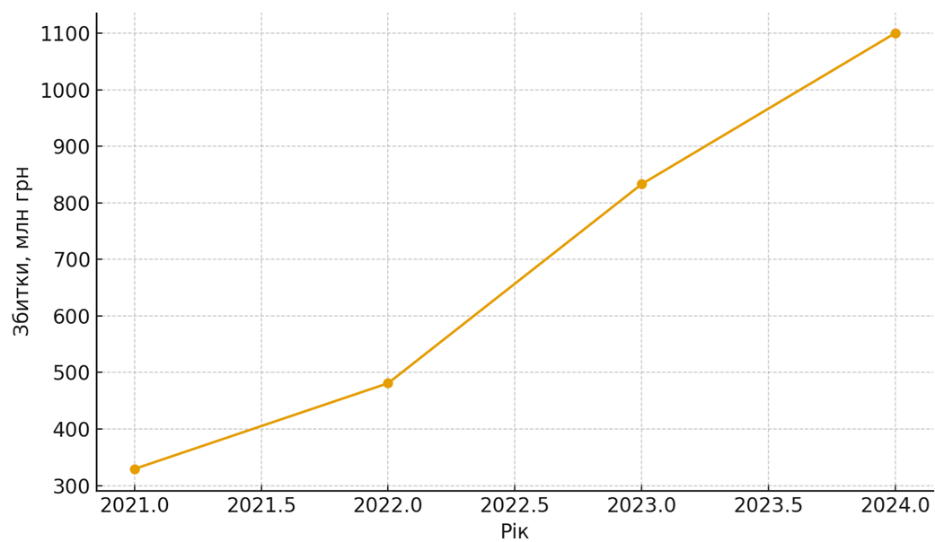
\includegraphics[width=0.9\linewidth]{img/figure1_1.png} 
    \caption{Збитки від шахрайств з платіжними картками в Україні}
    \label{fig:1_1}
\end{figure}

\newpage

На рис.~\ref{fig:1_1} показано лінійну динаміку збитків від незаконних дій з платіжними картками в Україні за 2021--2024~рр., яка була побудована автором на основі власних розрахунків та досліджень. Візуально видно рівень втрат, а подальше збільшення в 2024-му корелює з поширенням соціальної інженерії та зростанням середнього чека однієї незаконної операції. Це підтверджує ключову тезу розділу: шахрайство трансформувалося у системний бізнес, який базується не стільки на технічних вразливостях систем, скільки на маніпулюванні людським фактором і помилках користувачів~\cite{NBU2025}.

\vspace{0.3cm}
\section{Що найчастіше працює у шахраїв?}

Типові афери залишаються простими, але масовими. Найбільш поширені сценарії включають передоплату за товар, якого не існує, або «неймовірно вигідні» пропозиції від щойно створених акаунтів. Другою за масштабом схемою є сайти-двійники сервісу «OLX Доставка», які копіюють дизайн оригінальної сторінки й збирають реквізити карток під приводом «підтвердження доставки». 

А ще активно застосовуються цифрові псевдопослуги: фейкові страхування, оплата комуналки чи «швидкі кредити», де людина добровільно вводить персональні дані. Статистика демонструє, що вартість кожної атаки стрімко зростає. Середня сума шахрайської операції в інтернеті у 2024~році становила 4~761~грн, тоді як у 2023-му вона складала лише 3~150~грн. Більш того, у випадках довготривалого «ведення клієнта» (соціальна інженерія) шахраї виманювали в середньому 8~500~грн за одну оборудку. Це підтверджує, що шахрайство давно переросло дрібні випадкові крадіжки й перетворилося на бізнес-модель із власною економікою~\cite{NBU2025}.

\vspace{0.3cm}
\section{Чому люди «ведуться»?}

Зловмисники створюють ефект надпривабливості: пропозиція виглядає настільки вигідною, що мозок підсвідомо прагне уникнути втрати такого шансу. Далі активується штучний дефіцит часу: вимоги на кшталт «акція діє лише годину» або «підтвердіть оплату за 10 хвилин» блокують префронтальну кору, яка відповідає за логічний аналіз, і змушують діяти на рівні швидких реакцій. І нарешті, спрацьовує ефект соціального доказу: коли ми бачимо позитивний досвід інших у вигляді численних відгуків чи високих рейтингів (які часто є фальшивими), наш мозок автоматично маркує ситуацію як безпечну. Це нормальний еволюційний механізм орієнтації в соціумі, який шахраї використовують проти нас, щоб вимкнути раціональну перевірку фактів.

\chapter{Правова кваліфікація дій кібершахраїв}

Законодавство України передбачає комплексну відповідальність за шахрайські дії в цифровому просторі.

Згідно з Кримінальним кодексом України (ККУ), дії зловмисників кваліфікуються за кількома статтями залежно від методу вчинення злочину~\cite{CriminalCode}:

\begin{description}
    \item[ст. 190 (Шахрайство)] — заволодіння чужим майном або придбання права на майно шляхом обману чи зловживання довірою;
    
    \item[ст. 361] — несанкціоноване втручання в роботу інформаційних (автоматизованих), електронних комунікаційних мереж (застосовується у випадках технічного зламу або використання вразливостей систем);
    
    \item[ст. 361-1] — створення з метою протиправного використання, розповсюдження або збуту шкідливих програмних чи технічних засобів, а також їх розповсюдження;
    
    \item[ст. 361-2] — несанкціоновані збут або розповсюдження інформації з обмеженим доступом, яка зберігається в електронно-обчислювальних машинах (зокрема, бази даних платіжних карток, логінів та паролів).
\end{description}

\newpage

Окрім кримінального переслідування, важливу роль відіграють цивільно-правові наслідки використання чужих брендів, дизайнів та інтерфейсів для створення фішингових ресурсів. Цивільний кодекс України гарантує судовий захист прав інтелектуальної власності (ст.~432) та встановлює відповідальність за їх порушення (ст.~431)~\cite{CivilCode}.

\vspace{0.3cm}

Спеціальне законодавство деталізує ці норми:

\begin{enumerate}
    \item Закон України «Про охорону прав на знаки для товарів і послуг» визначає виключні права власника бренду (ст.~16) та кваліфікує як порушення будь-яке посягання на них, зокрема імітацію знаку або введення споживачів в оману (ст.~20)~\cite{LawTrademarks}.
    
    \item Для охорони елементів дизайну, текстів та зображень застосовується Закон України «Про авторське право і суміжні права». Він передбачає механізми припинення порушень та стягнення компенсації, а також визначає відповідальність власників вебсайтів за невидалення піратського контенту після отримання відповідної скарги~\cite{LawCopyright}.
    
    \item У випадках, коли шахрайський ресурс (клон) маскується під оригінальний сервіс, застосовуються норми Закону «Про захист від недобросовісної конкуренції» (ст.~15-1) щодо заборони поширення інформації, що вводить в оману~\cite{LawCompetition}.
\end{enumerate}

У судовій практиці для потерпілої сторони (наприклад, банку чи маркетплейсу) ключовим є доведення факту порушення прав інтелектуальної власності для застосування цивільних засобів захисту, що відбувається паралельно з фіксацією ознак шахрайства у межах кримінального провадження.

\vspace{0.3cm}
\noindent\textbf{Статистичні тенденції та висновки}

Порівняльний аналіз статистичних даних демонструє тривожну динаміку: від 481~млн гривень втрат у 2021~році до понад 1,1~млрд~грн у 2024-му. Це свідчить про те, що кібершахрайство перестало бути сукупністю поодиноких інцидентів і трансформувалося у системне явище, темпи розвитку якого випереджають ріст цифрової грамотності суспільства~\cite{NBU2025}.

У контексті платформ оголошень і псевдопослуг ключовою вразливістю є не слабкість технологій захисту, а людський фактор: надмірна довіра, поспіх та відсутність критичного мислення. 

За даними регулятора, саме соціальна інженерія стала причиною 93\% усіх фінансових втрат в інтернеті. Тут діє головне правило: чим привабливішою та «яскравішою» виглядає пропозиція, тим вища ймовірність, що це — ретельно підготовлена пастка~\cite{NBU2025}.

\chapter{Ознаки шахрайських пропозицій}

Найперший тригер\footnote{Первинний сигнал, який запускає настороженість і спонукає зупинитися та перевірити.} — занадто низька ціна або пропозиція, що виглядає «занадто вигідною». Шахраї навмисне ставлять вартість нижчу за ринкову, щоб спровокувати покупця діяти імпульсивно, наприклад демпінг\footnote{Від англ. dumping. Продаж товарів за цінами, нижчими від собівартості.} у 30--50\%. Коли людина бачить смартфон, ноутбук чи павербанк\footnote{Портативний зовнішній акумулятор, який дозволяє заряджати ваші електронні пристрої.} на третину дешевше, ніж у магазинах, мозок миттєво фіксує «вигоду» і відсуває сумніви на другий план (рис.~\ref{fig:1_2}). Технічно для шахрая це працює як приманка: оголошення створюється за кілька хвилин, а вже далі все тримається на психології довірливості. Кіберполіція України офіційно визначає цю ознаку як ключовий індикатор небезпеки. Правоохоронці застерігають: якщо ціна товару суттєво відрізняється від середньої ринкової ціни на аналогічні моделі (різниця понад 20--30\%), ймовірність шахрайства наближається до 100\%~\cite{CyberpoliceTips}.

% Параметр [H] змушує рисунок бути САМЕ ТУТ, а не <<десь на сторінці>>
\begin{figure}[H]
    \centering
    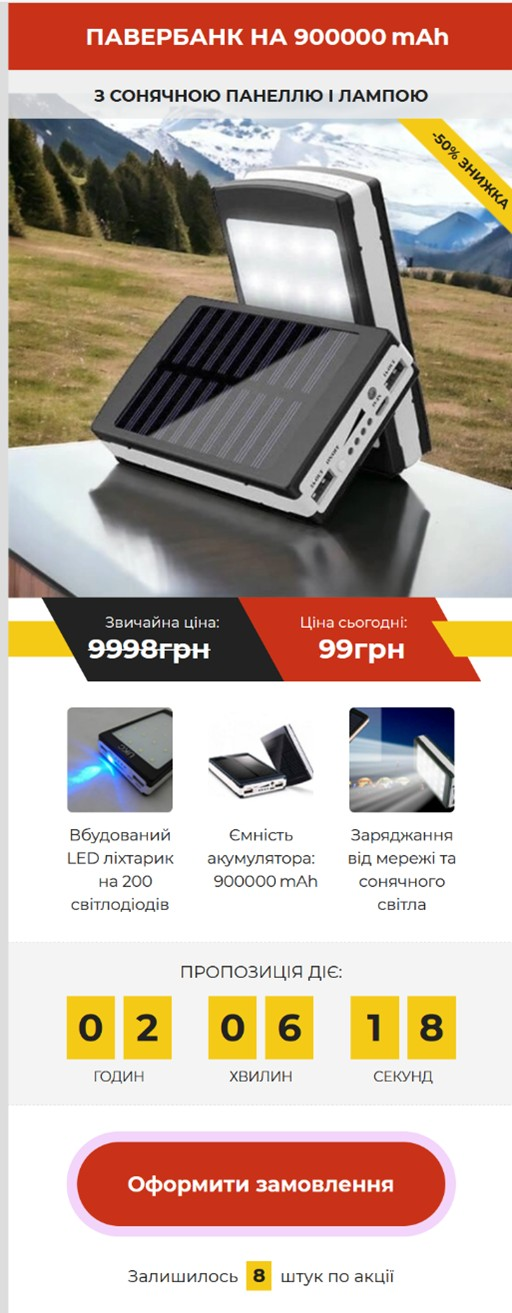
\includegraphics[width=0.50\linewidth]{img/figure1_2.jpg} 
    \caption{Приклад фейкової реклами на маркетплейсах}
    \label{fig:1_2}
\end{figure}

Зверніть увагу на технічні характеристики (рис.~\ref{fig:1_2}). Вказана на рекламному банері ємність у 900 000 mAh є фізично неможливою для пристрою такого розміру. 

Для порівняння: стандартний зовнішній акумулятор на 20 000 mAh важить близько 400–500 грамів. Повербанк ємністю 900 000 mAh мав би важити понад 15–20 кілограмів і за розмірами нагадував би автомобільний акумулятор або велику валізу. Використання таких «космічних» цифр — це пряма ознака шахрайства, розрахована на неуважність або технічну необізнаність покупця.

\vspace{0.3cm}
\noindent\textbf{Відсутність можливості зустрітися}

Ще однією характерною ознакою є відсутність можливості зустрітися особисто чи оглянути товар перед покупкою. Продавець знаходить «поважні причини»: мовляв, перебуває у відрядженні, товар зберігається на складі або він уже запакований для відправки. Така поведінка технічно дозволяє шахраю залишатися анонімним: йому не треба демонструвати фізичний товар, достатньо лише підтримувати контакт через месенджер. Це також спрощує використання фейкових фото, які легко взяти з інтернету.

\vspace{0.3cm}
\noindent\textbf{Вимога термінової передоплати}

Надзвичайно поширеним є прийом вимоги термінової передоплати. Класичне формулювання — «зараз або ніколи»: «ще кілька охочих чекають», «бронюю тільки після авансу». Тут шахрай використовує технічний інструмент — переказ на банківську картку чи електронний гаманець. У більш просунутих випадках надсилається покликання на підроблений сайт, що імітує платіжний сервіс. У цьому випадку користувач сам вводить дані своєї картки на фішинговій сторінці, після чого злочинець отримує прямий доступ до рахунку.

\vspace{0.3cm}

\newpage

\noindent\textbf{Некоректні або крадені фотографії}

Ще одна явна ознака — некоректні або крадені фотографії. Шахраї рідко мають справжній товар, тому беруть зображення з Google Images, Instagram чи офіційних сайтів виробників. Технічно це легко перевірити: достатньо завантажити фото в Google і знайти десятки ідентичних картинок у чужих оголошеннях. Це простий, але дієвий спосіб викрити шахрайство.

\vspace{0.3cm}
\noindent\textbf{Новостворений профіль}

Важливим показником є й новостворений профіль без історії чи з фейковими відгуками. Зловмисники відкривають акаунт, виставляють кілька «товарів», а щоб виглядати переконливо, підробляють коментарі — залишають штучні відгуки зі сторонніх акаунтів. Технічно це робиться через реєстрацію декількох профілів на один номер, через віртуальні SIM-карти чи тимчасові email-адреси (див. табл.~\ref{tab:table2}). Після того як профіль викривають і блокують, шахрай легко створює новий, повторюючи схему.

\newpage

\noindent Як це виглядає на практиці:


\begin{table}[H]
    \centering
    \caption{Маркери фейкових оголошень}
    \label{tab:table2}
    % Розподіл ширини колонок: 25%, 35%, 30% сторінки
    \begin{tabular}{|>{\raggedright\arraybackslash}p{0.23\linewidth}|>{\raggedright\arraybackslash}p{0.33\linewidth}|>{\raggedright\arraybackslash}p{0.28\linewidth}|}
        \hline
        \multicolumn{1}{|c|}{\textbf{Ознака}} & \multicolumn{1}{c|}{\textbf{Як працює технічно}} & \multicolumn{1}{c|}{\textbf{Чому діє психологічно}} \\ \hline
        
        Підозріло низька ціна & 
        Оголошення створюється з демпінгом (30--50\% від ринку), фото й опис беруться з інтернету & 
        Викликає відчуття «вигоди», знижує критичність, стимулює діяти швидко \\ \hline
        
        Відсутність зустрічі чи огляду & 
        Продавець вигадує причини: відрядження, склад, «товар запакований» & 
        Створює ілюзію раціональності: пояснення виглядають логічними і знижують пильність \\ \hline
        
        Вимога термінової передоплати & 
        Переказ на карту або покликання на фішинговий сайт, що імітує банк & 
        Тиск часу («зараз або ніколи») змушує приймати рішення імпульсивно \\ \hline
        
        Фейковi або чужi фотоо & 
        Зображення беруться з вiдкритих джерел & 
        Довіра до візуальних образів: якісні фото асоціюються з надійністю продавця \\ \hline
        
        Новостворений профіль без історії & 
        Реєстрацiя через тимчасовi данi, штучнi вiдгуки & 
        Маніпуляція соціальним доказом: створюється хибне відчуття безпечного середовища \\ \hline
    \end{tabular}
\end{table}

Таким чином, шахрайські пропозиції поєднують психологічний тиск (вигода, терміновість, довіра) з технічними прийомами (фейкові сайти, крадені фото, нові акаунти, підроблені відгуки). Для користувача важливо розуміти: якщо хоча б один із цих сигналів присутній, угоду варто перевіряти вдвічі ретельніше або взагалі відмовитися від неї.

Перевіряйте контакти таких покупців через спеціалізовані інструменти, наприклад GetContact або пошук у Google, а покликання — на VirusTotal, PhishTank (див. підрозділ~1.10).

\chapter{Інструменти для перевірки продавців та покупців}

Шахраї розраховують, що ви не перевірятимете. Перевірка — ваш найкращий щит.

\vspace{0.3cm}
\noindent\textbf{Чек-лист швидкої перевірки}

Щоб уникнути шахрайства під час онлайн-угод, головне правило – ніколи не здійснюйте передоплату незнайомим користувачам. Навіть невелика сума може бути втрачена, якщо оголошення фейкове. Безпечніше зустрітися особисто або скористатися оплатою при отриманні.

\vspace{0.3cm}
\noindent\textbf{Перевірка профілю}

Звертайте увагу на:
\begin{enumerate}
    \item \textbf{Дату реєстрації} — нові акаунти часто шахрайські.
    \item \textbf{Кількість і тематику оголошень} — якщо активність мінімальна або надто різнопланова, це сигнал ризику.
    \item \textbf{Відгуки} — реальні користувачі залишають конкретні коментарі, а не загальні «все добре».
    \item \textbf{Поведінку} — надмірна терміновість, надто вигідні умови чи готовність купити без огляду товару —  тригери обману.
\end{enumerate}

\newpage

\noindent\textbf{Перевірка зображень і контактів:}

\begin{enumerate}
    \item Перевіряйте фото товару через \textbf{Google Images}: якщо фото з’являється на інших сайтах, товар, ймовірно, неіснуючий.
    \item Шукайте номер телефону або email у \textbf{Google}, \textbf{Bing}, \textbf{WhoCallsMe.net}, \textbf{Truecaller.com} чи додатку \textbf{GetContact} — він часто показує, як інші користувачі зберегли цей номер («шахрай», «OLX доставка» тощо).
\end{enumerate}

\vspace{0.3cm}
\noindent\textbf{Перевірка платіжних реквізитів}

Якщо продавець просить передоплату, перевірте його картку через:
\begin{enumerate}
    \item \texttt{cyberpolice.gov.ua} — розділ «Stop Fraud» (або «Перевірити картку»).
    \item \texttt{ema.com.ua} (StopFraud) — база шахрайських рахунків.
    \item Перевірка IBAN на \texttt{bank.gov.ua} — дозволяє підтвердити належність рахунку банку.
\end{enumerate}

\vspace{0.3cm}
\noindent\textbf{Перевірка покликань}

Ніколи не переходьте за покликанням з месенджерів або SMS. Перевіряйте отримані URL\footnote{Текст зазвичай синього кольору, на який можна натиснути, щоб перейти на інший сайт.} через:
\begin{enumerate}
    \item \texttt{VirusTotal.com} — аналіз сайтів і файлів.
    \item \texttt{PhishTank.com} — база фішингових сторінок.
    \item \texttt{Whois.domaintools.com} — перевірка домену (дати реєстрації, власника).
\end{enumerate}

\newpage

Експерти Асоціації ЄМА наголошують: шахраї часто намагаються вивести спілкування з офіційної платформи в месенджери (Viber, Telegram), щоб надіслати фішингове покликання. Для перевірки будь-якого покликання, отриманого від продавця чи покупця, використовуйте сервіс \textbf{CheckMyLink} (\texttt{https://check.ema.com.ua/}).

Цей інструмент (рис.~\ref{fig:1_3}) перезвіряє покликання із загальноукраїнською базою шахрайських ресурсів та попереджає про небезпеку ще до моменту переходу на сайт~\cite{EMACheck}.

\begin{figure}[H]
    \centering
    % Переконайтеся, що файл називається fig1_3 (jpg/png) і лежить в папці img
    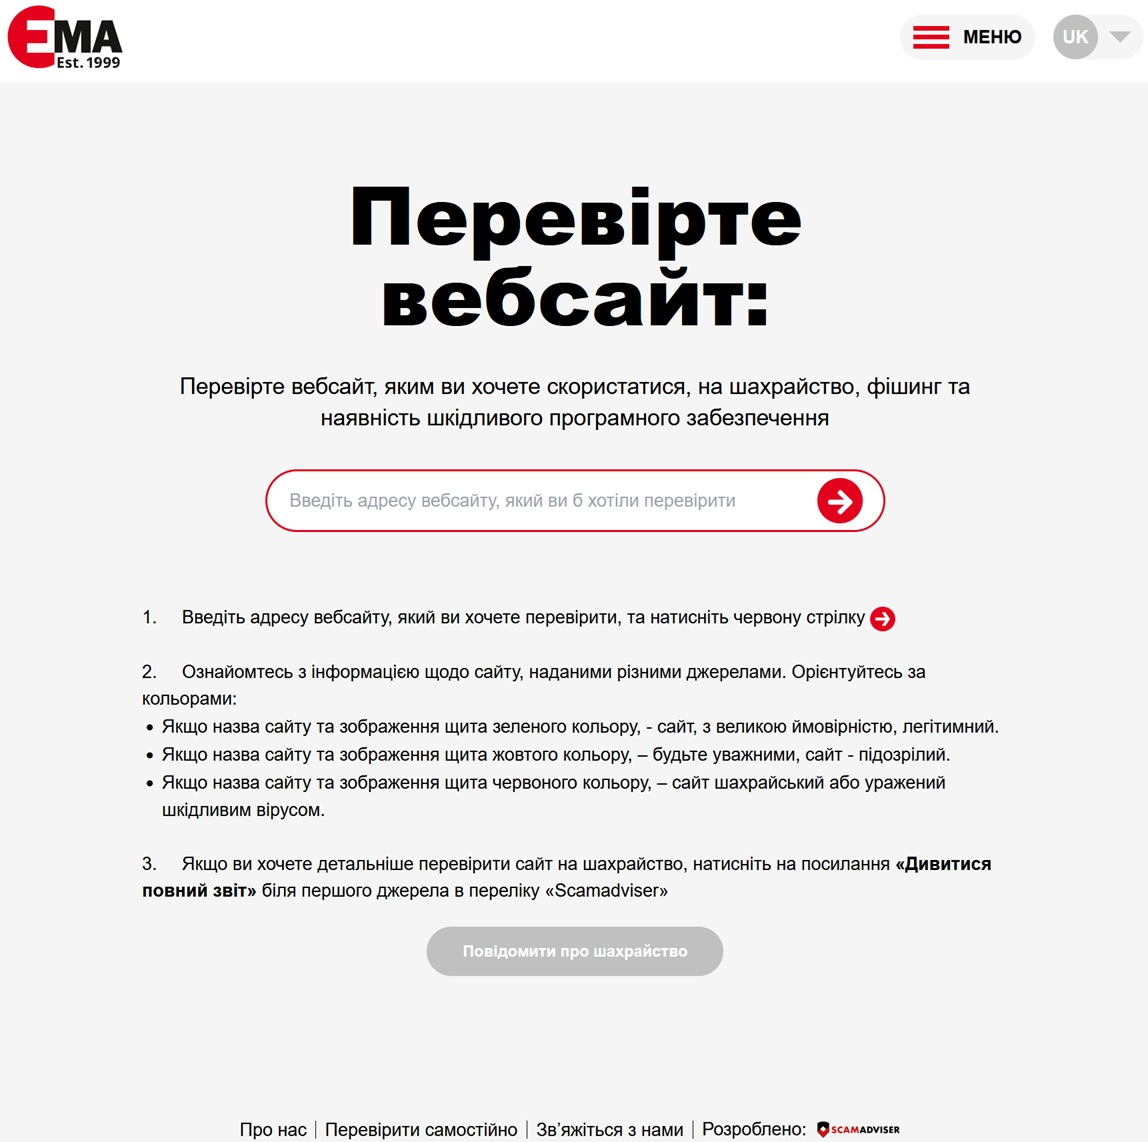
\includegraphics[width=0.75\linewidth]{img/figure1_3.jpg} 
    \caption{Вікно з перевіркою вебсайту на платформі ЄМА}
    \label{fig:1_3}
\end{figure}

Якщо сервіс показує, що сайт підозрілий або шахрайський, негайно припиніть спілкування.

\newpage

\chapter{Поради щодо захисту та дії у випадку шахрайства}

Безпечна угода — це не удача, а звичка. Щоб уникнути фінансових втрат і зберегти особисті дані, важливо не лише знати типові схеми шахраїв, а й діяти за чітким алгоритмом безпеки.

\section{Алгоритм безпечної угоди}

\vspace{0.3cm}
\noindent\textbf{Алгоритм безпечної угоди: як не стати жертвою шахраїв}

\begin{enumerate}
    \item \textbf{Всебічно перевіряйте контрагента.} Дивіться дату реєстрації профілю, кількість оголошень та відгуки (нові або «порожні» акаунти — сигнал ризику). Перевіряйте номер телефону, email або картку в Google, GetContact чи StopFraud. Зробіть зворотний пошук фото — якщо зображення крадені, це шахрай.
    
    \item \textbf{Користуйтеся лише офіційними сервісами.} Оплачуйте через вбудовані інструменти платформи (як «OLX Доставка») або інші надійні сервіси. Ніколи не переказуйте гроші напряму на картку невідомої особи.
    
    \item \textbf{Дотримуйтесь базової кібергігієни} (правила чистоти та безпеки в інтернеті). Увімкніть двофакторну автентифікацію (2FA), створюйте унікальні паролі та використовуйте окрему картку з лімітом для онлайн-платежів. Спілкуйтеся лише в офіційних чатах платформи.
    
\newpage

    \item \textbf{Вимагайте документи для дорогих покупок.} Для оренди чи купівлі нерухомості або авто вимагайте документи та звіряйте їх через офіційні державні реєстри.
    
    \item \textbf{Довіряйте здоровому глузду.} Якщо ціна занадто приваблива, продавець уникає дзвінків, поспішає або надто наполегливо вимагає передоплату — привід зупинити угоду. Якщо щось викликає сумнів — краще втратити можливу вигоду, ніж гроші та дані.
    
    \item \textbf{Зберігайте докази.} Якщо угода відбулася, збережіть усе: контакти, квитанції, чеки та повну історію листування.
\end{enumerate}

\section{Алгоритм дій. Що робити, якщо вас ошукали?}

Якщо ви зрозуміли, що передали дані шахраям або з вашого рахунку зникли гроші, ви можете відчути сильний сором, гнів або самозвинувачення. \textbf{Зупиніться.} Ваша реакція (паніка, прискорене серцебиття) є абсолютно нормальною відповіддю організму на гострий стрес. Пам’ятайте: те, що сталося — це результат застосування професійних технік психологічного тиску, а не ваша «провина» чи «наївність». Зараз час — ваш головний союзник, але діяти потрібно миттєво. Не дозволяйте емоціям заблокувати вашу рішучість. Поверніть собі контроль над ситуацією через ці чіткі кроки:

\begin{enumerate}
    \item \textbf{Заблокуйте банківську картку (НЕГАЙНО).}
    Це найперший крок, щоб шахраї не встигли зняти решту грошей.
    \begin{itemize}
        \item \textbf{Спосіб 1. Через мобільний застосунок.} Відкрийте програму вашого банку (Приват24, monobank, Ощад тощо) на телефоні. Знайдіть зображення вашої картки, натисніть на нього або на меню «Налаштування» (шестерня) і оберіть пункт \textbf{«Заблокувати картку»}.
   \newpage
   
        \item \textbf{Спосіб 2. Через гарячу лінію.} Якщо у вас немає застосунку або інтернету, терміново телефонуйте в банк.
        \item \textit{Де знайти номер?} Номер гарячої лінії завжди написаний \textbf{на зворотному боці вашої пластикової картки} (зазвичай починається на 0-800...). Також його можна знайти на офіційному сайті банку.
        \item \textit{Що казати?} «Я підозрюю шахрайство, терміново заблокуйте мої рахунки».
    \end{itemize}

    \item \textbf{Зверніться до банку офіційно.}
    Дзвінка недостатньо. Вам потрібно зафіксувати факт злочину документально.
    \begin{itemize}
        \item Зателефонуйте на гарячу лінію та повідомте оператору про крадіжку коштів.
        \item Вимагайте сформувати заявку на \textbf{повернення коштів} (процедура оскарження транзакції).
        \item Найближчим часом відвідайте відділення банку та напишіть письмову \textbf{заяву про несанкціоновану операцію}. Обов'язково попросіть копію цієї заяви з відміткою банку про отримання. Це ваш доказ для поліції та суду.
    \end{itemize}

    \item \textbf{Зберіть докази злочину.}
    Поки ви чекаєте на відповідь банку, збережіть усе, що стосується шахраїв. Потім вони можуть видалити листування.
    \begin{itemize}
        \item \textbf{Скріншоти (знімки екрана).} Сфотографуйте листування у месенджерах (Viber, Telegram), SMS-повідомлення, сторінку шахрайського сайту чи профілю продавця.
        \item \textbf{Фінансові дані.} Збережіть квитанції про переказ, номер картки, на яку ви скидали гроші, та точний час операції.
        \item \textbf{Контакти.} Запишіть номери телефонів, з яких вам дзвонили, та нікнейми (імена) шахраїв в інтернеті.
    \end{itemize}

    \item \textbf{Подайте заяву до Кіберполіції.}
    Не думайте, що «через 500 гривень ніхто не шукатиме». Ваша заява може стати частиною великої справи проти злочинної групи.
    \begin{itemize}
        \item \textbf{Варіант А (Онлайн, найшвидше).} Зайдіть на сайт Кіберполіції \url{https://ticket.cyberpolice.gov.ua/} та заповніть електронну форму «Повідомити про злочин».
        \item \textbf{Варіант Б (Особисто).} Підіть у найближче відділення поліції та напишіть заяву про вчинення кримінального правопорушення за статтею 190 ККУ (Шахрайство). Додайте до заяви роздруковані скріншоти та копії квитанцій.
    \end{itemize}
\end{enumerate}

\vspace{0.2cm}
\textit{\textbf{Пам'ятайте.} Банк ніколи не дзвонить, щоб запитати PIN-код, пароль від входу в кабінет або три цифри на звороті картки (CVV). Якщо вас про це запитують — це шахраї. Кладіть слухавку і дзвоніть у банк самі за номером на вашій картці.}

\clearpage